\documentclass[12pt]{report} 

% PACKAGES 
\usepackage[dutch]{babel}
\usepackage[utf8]{inputenc}
\usepackage{color}
\usepackage{amsmath} % Matrices
\usepackage{amsfonts}
\usepackage{enumitem}
\usepackage{booktabs}
\usepackage{xcolor}
\usepackage{sectsty}
\usepackage{graphicx}
\usepackage{lipsum}

\graphicspath{{img/}}

\newcommand{\answercolor}{teal}


\partfont{\color{brown}}
\chapterfont{\color{teal}}
\sectionfont{\color{cyan}}

% DOCUMENT INFORMATION
\title{Wiskunde A}
\author{Bert De Saffel}
\date{2017-2018}


% CUSTOM COMMANDS
\newcommand{\todo}[1] {
\color{red}\textunderscore{\textit{TODO: #1}}
}

\newcommand{\important}[1] {\textbf{\color{orange}#1}}
\newcommand{\mathimportant}[2] {\textbf{\color{#2}$#1$}}

% DOCUMENT
\begin{document}
\maketitle
\tableofcontents

\part{Theorie}
\chapter{Complexe Getallen}
\important{Inleiding}
\begin{itemize}
 \item $\mathbb{N}$ = Natuurlijke getallen: \{0, 1, 2, 3, ...\}
 \item $\mathbb{Z}$ = Gehele getallen: \{..., -2, -1, 0, 1, 2, ...\}
 \item $\mathbb{Q}$ = Rationale getallen: \{$\frac{1}{3}$, $-\frac{1}{4}$, $\frac{7}{2}$, ... \}
 \item $\mathbb{R}$ = Reële getallen: \{ $\sqrt{2}$ , $\pi$ \}
 \item $\mathbb{C}$ = Complexe getallen: $j^2 = -1$, $j = $ imaginaire eenheid
\end{itemize}
\important{Definitie}
$z = \mathimportant{a}{orange} + \mathimportant{b}{orange}j$ met $z \in \mathbb{C}$, $a \in \mathbb{R}, b \in \mathbb{R}$ en $j = \sqrt{-1}$ met
\begin{itemize}
 \item $Re(z) = a$
 \item $Im(z) = b$
\end{itemize}
\important{3 Vormen}
\begin{itemize}
 \item Cartesische vorm: $z = a + bj$
 \item Goniometrische vorm: $z = r[cos(\theta) + jsin(\theta)]$
 \item Exponentiële vorm: $re^{j\theta}$
\end{itemize}
\important{Vlak van Gauss}
\begin{itemize}[label={}]
 \item 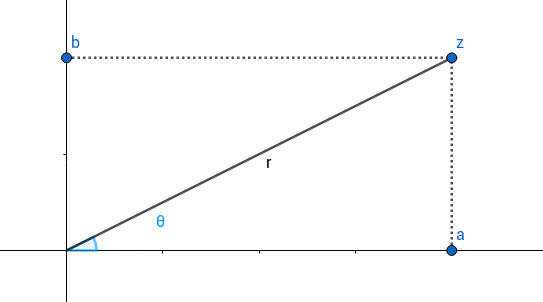
\includegraphics[width=\linewidth]{goniometrischevorm}
\end{itemize}
\important{a en b}
\begin{itemize}
 \item $a = rcos(\theta)$
 \item $b = rsin(\theta)$
\end{itemize}
\important{r en $\theta$}
\begin{itemize}
 \item $r \geq 0$
 \item $r = \sqrt{a^2 + b^2}$
 
 \item $\theta \in [0, 2\pi]$
 \item $\theta \in ]-\pi, \pi[$
 \item $tg(\theta) = \frac{b}{a} (+ \pi)$
\end{itemize}
\important{Complex toegevoegde}
\begin{itemize}
 \item Cartesische vorm: $\overline{z} = a - bj$ 
 \item Exponentiële vorm: $\overline{z} = re^{-j\theta}$
\end{itemize}
\important{Bewerkingen}
\begin{itemize}
 \item $z_1 + z_2$
 \item $z_1 . z_2 = (r_1 . r_2)e^{j(\theta_1 + \theta_2)}$
 \item $\frac{z_1}{z_2} = \frac{r_1}{r_2}e^{j(\theta_1 - \theta_2)}$
 \item $z^{n} = r^{n}e^{jn\theta}$
 \item $\sqrt[n]{z} = r^{\frac{1}{n}}e^{j\frac{1}{n}}(\theta + 2k\pi)$
\end{itemize}
\end{document}
